\chapter{Results and Discussion}
\label{chap:results}

\par This chapter reports the experimental results of the methodology presented in Chapter~\ref{chap:ml_methodology}: data ingestion statistics, exploratory data analysis findings that shaped the feature set, model training dynamics, and classification performance across the two evaluated granularities (binary and 8-class attack-family) on the random split. It closes with a cross-model comparison and a discussion of the observed generalisation behaviour. The performance targets referenced here (NFR-2 and NFR-5) are formalised in the requirements of the application, in Section~\ref{sec:non_functional_requirements}.

\section{Data Ingestion and Class Distribution}
\label{sec:ingestion_results}

\par The ingestion pipeline processed all 34 CICIoT2023 source folders (the 33 attack types plus benign) and applied deduplication followed by per-class subsampling at a cap of 200{,}000 rows per fine-grained class. Figure~\ref{fig:ingest_waterfall} summarises the row counts at each stage.

\begin{figure}[htbp]
    \centering
    \begin{minipage}[t]{0.48\textwidth}
        \centering
        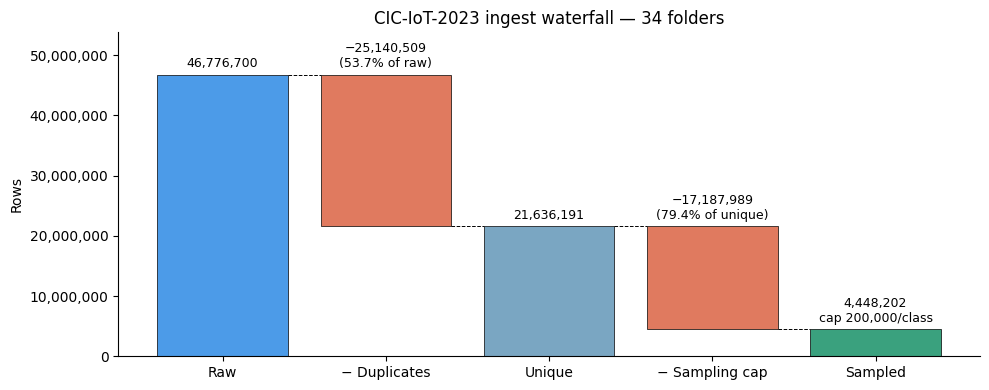
\includegraphics[width=\textwidth]{figures/ingest_waterfall.png}
        \caption{CICIoT2023 data reduction waterfall: raw records, exact duplicates removed, per-class cap applied, and the resulting working set.}
        \label{fig:ingest_waterfall}
    \end{minipage}\hfill
    \begin{minipage}[t]{0.48\textwidth}
        \centering
        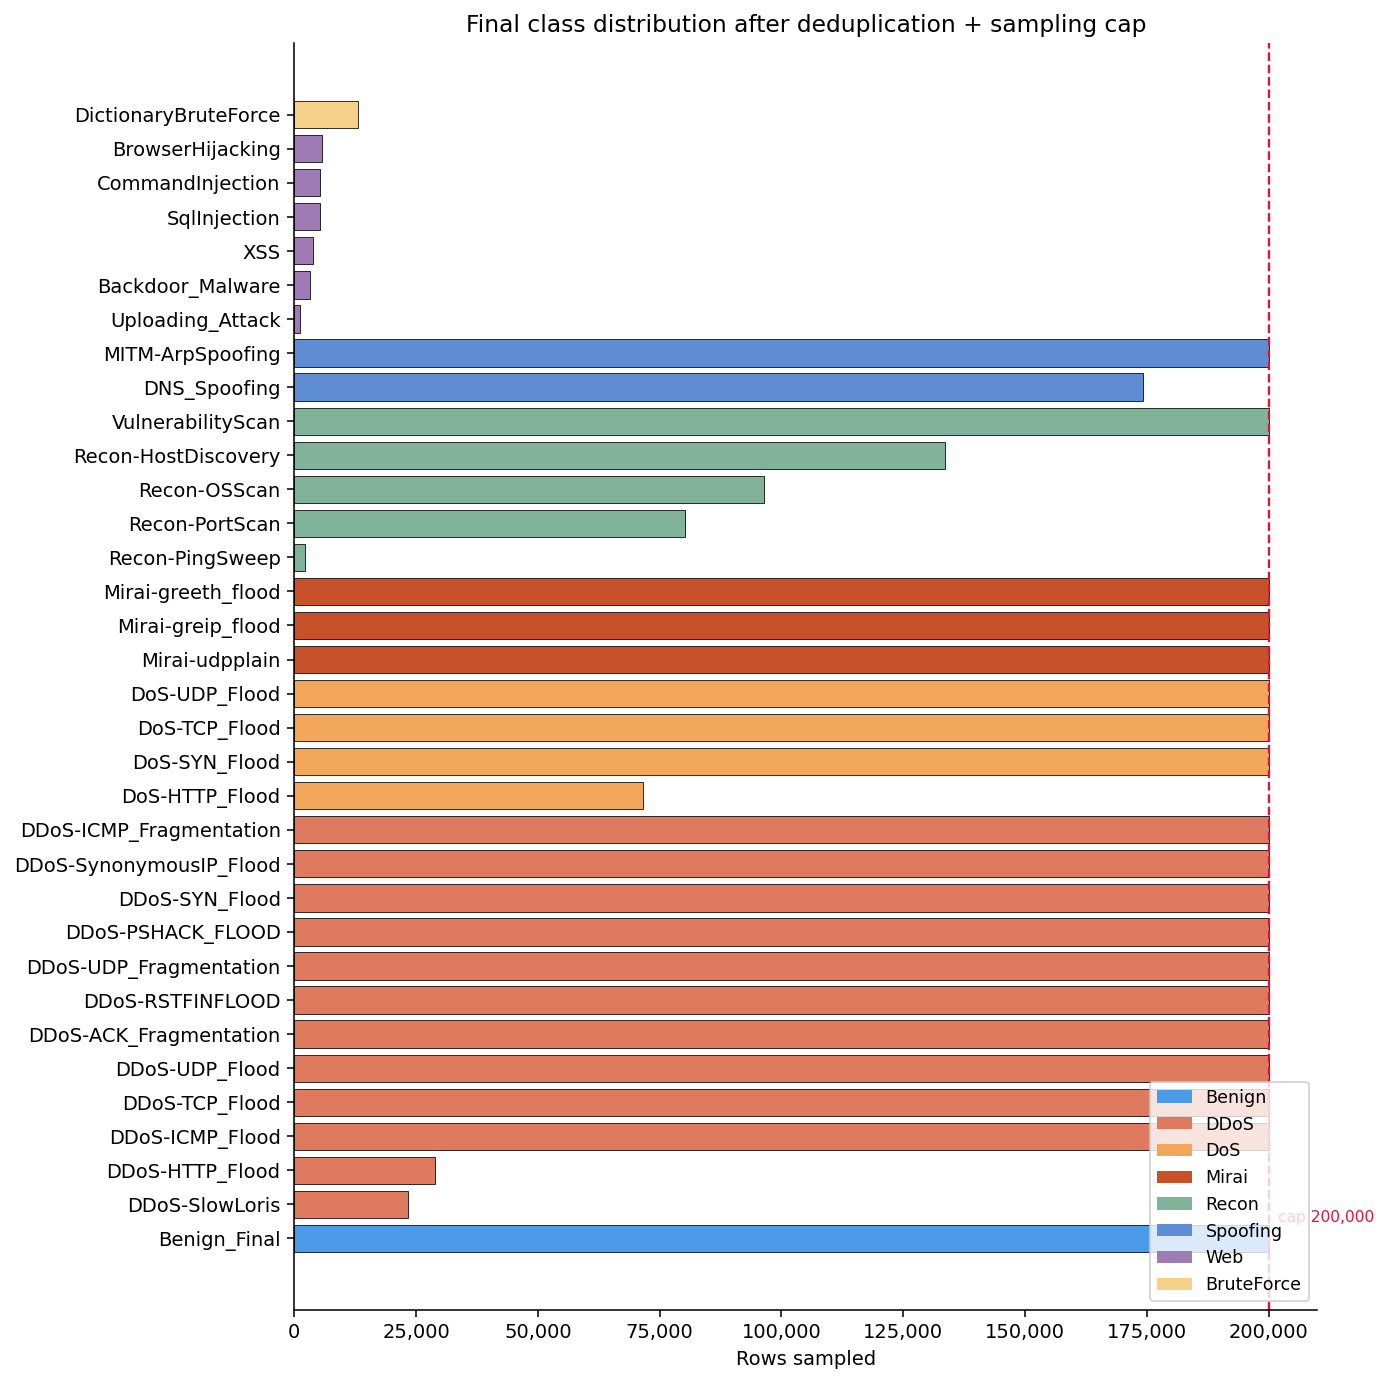
\includegraphics[width=\textwidth]{figures/dist_class_bar.png}
        \caption{Final class distribution across the 34 fine-grained labels after deduplication and sampling; the dashed line marks the per-class cap.}
        \label{fig:dist_class_bar}
    \end{minipage}
\end{figure}

\par The waterfall (Figure~\ref{fig:ingest_waterfall}) reduces the 46{,}776{,}700 raw records to a 4{,}448{,}202-row working set in two stages, and two features of this reduction matter. First, the duplicate fraction is unusually high: 53.7\% of the raw records are byte-identical to another row in the same folder. This is a known property of the dataset and has been reported by other authors \cite{CICIoT2023}. Deduplicating before sampling is therefore critical: without this step, each sampled row would carry implicit near-duplicate neighbours, inflating test accuracy to an optimistic and meaningless level. Second, the 200{,}000-row-per-class cap then discards 79.4\% of the 21{,}636{,}191 unique rows, but it only limits the large classes. After deduplication the majority class (DDoS-ICMP\_Flood) still has over 200{,}000 unique rows, so the cap reduces it to 200{,}000, whereas the rarest web-based attacks (XSS, Backdoor\_Malware, CommandInjection) have fewer than 5{,}000 unique rows each, far below the cap, so they are kept in full. The cap therefore narrows the imbalance between the largest and smallest classes but does not remove it.

\par Figure~\ref{fig:dist_class_bar} shows the class distribution after deduplication and sampling at the fine-grained 34-class level. Grouped into the eight attack families, the same working set is dominated by DDoS at 46.1\%, followed by DoS (15.1\%), Mirai (13.5\%), and Reconnaissance (11.5\%), with Benign at only 4.5\% and the web-based family below 1\%. The volumetric families sit at the cap while the rare web-based attacks fall far below it, which reflects the original dataset imbalance rather than the sampling cap.

\section{Exploratory Data Analysis}
\label{sec:eda_results}

\par Exploratory analysis informed two feature-set decisions: the removal of near-zero-variance binary features and the logging transform applied to heavy-tailed continuous features. The binary-flag variances were computed on the full cleaned dataset, while the continuous-feature correlations and the heavy-tail diagnostics used a 50{,}000-row random subsample; both were carried out before the train/validation/test split.

\subsection{Continuous Feature Correlations}
\label{subsec:correlations}

\par Figure~\ref{fig:pearson_corr} shows the Pearson correlation matrix of the 18 continuous features after the $\log(1+x)$ transform.

\begin{figure}[htbp]
    \centering
    \begin{minipage}[t]{0.48\textwidth}
        \centering
        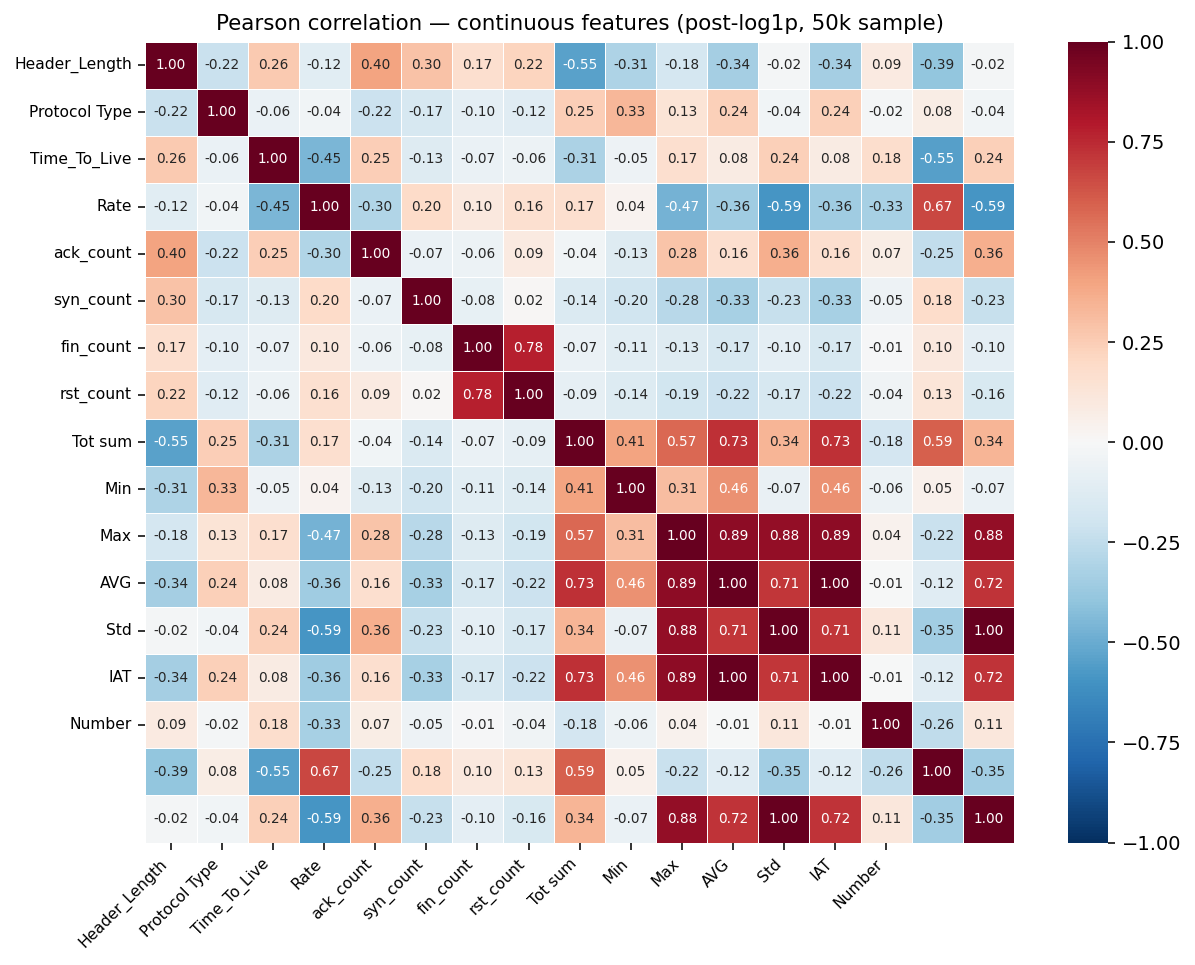
\includegraphics[width=\textwidth]{figures/pearson_corr.png}
        \caption{Pearson correlation matrix of the 18 continuous CICIoT2023 features on a 50{,}000-row post-log1p sample.}
        \label{fig:pearson_corr}
    \end{minipage}\hfill
    \begin{minipage}[t]{0.48\textwidth}
        \centering
        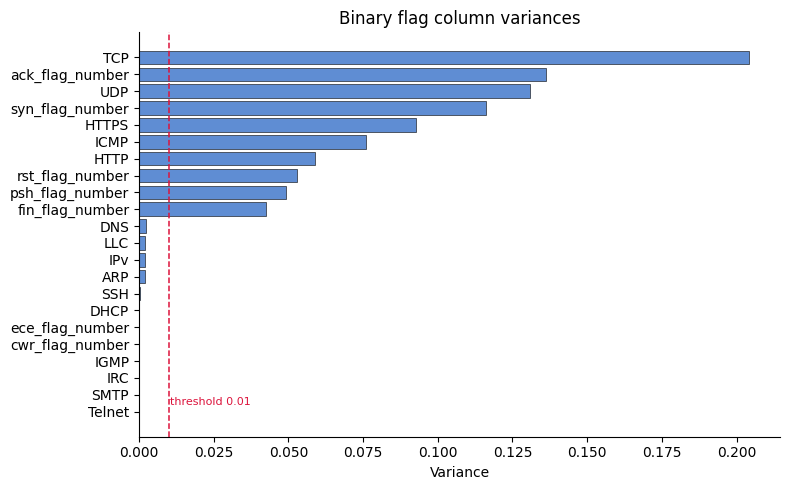
\includegraphics[width=\textwidth]{figures/flag_variances.png}
        \caption{Empirical variance of the 21 binary flag and protocol-indicator features, in descending order; the dashed red line marks the 0.01 threshold.}
        \label{fig:flag_variances}
    \end{minipage}
\end{figure}

\par Two perfectly collinear pairs are clearly visible: \texttt{AVG} packet length and \texttt{Tot\_size} (total bytes, which is average $\times$ count), and \texttt{Std} (standard deviation of packet lengths) and \texttt{Variance} (its square). From each pair the redundant member (\texttt{Tot\_size} and \texttt{Variance}) is dropped, keeping \texttt{AVG} and \texttt{Std}: the discarded column carries no information its partner does not, so a tree ensemble would select the same split point on either feature and the MLP is unaffected. The \texttt{IAT} (inter-arrival time) feature is nearly orthogonal to all others, which is consistent with its role as a timing feature rather than a size-based statistic.

\subsection{Binary Flag Feature Variance}
\label{subsec:flag_variances}

\par The 21 binary protocol-indicator and TCP flag columns vary widely in empirical variance. Figure~\ref{fig:flag_variances} shows these variances in descending order.

\par Features with variance below 0.01 are close-to-constant across the training sample and contribute noise rather than signal: a near-constant feature effectively tells the model nothing about class membership. Twelve such features are identified and removed. Together with the two redundant continuous columns dropped above, this prunes the set to the 25 features that form the input vector used by all models, ensuring that the scaler and the MLP are not exposed to the collinear or near-zero-variance columns that would otherwise require special handling.

\section{Feature Importance}
\label{sec:feature_importance}

\par Understanding \emph{which} features drive a model's decisions is a recurring concern in the explainable-AI-for-IDS literature, where post-hoc attribution is used to make deep detectors auditable rather than opaque (Section~\ref{subsec:xai_ids}) \cite{Almohri2024XAI}. To understand which of the 25 retained features carry the most discriminative weight, \emph{global} permutation importance (the drop in model performance when a single feature's values are randomly shuffled, breaking its association with the label) was computed on the Random Forest baseline. Figure~\ref{fig:feature_importance} shows the top 20 features by this importance score.

\begin{figure}[htbp]
    \centering
    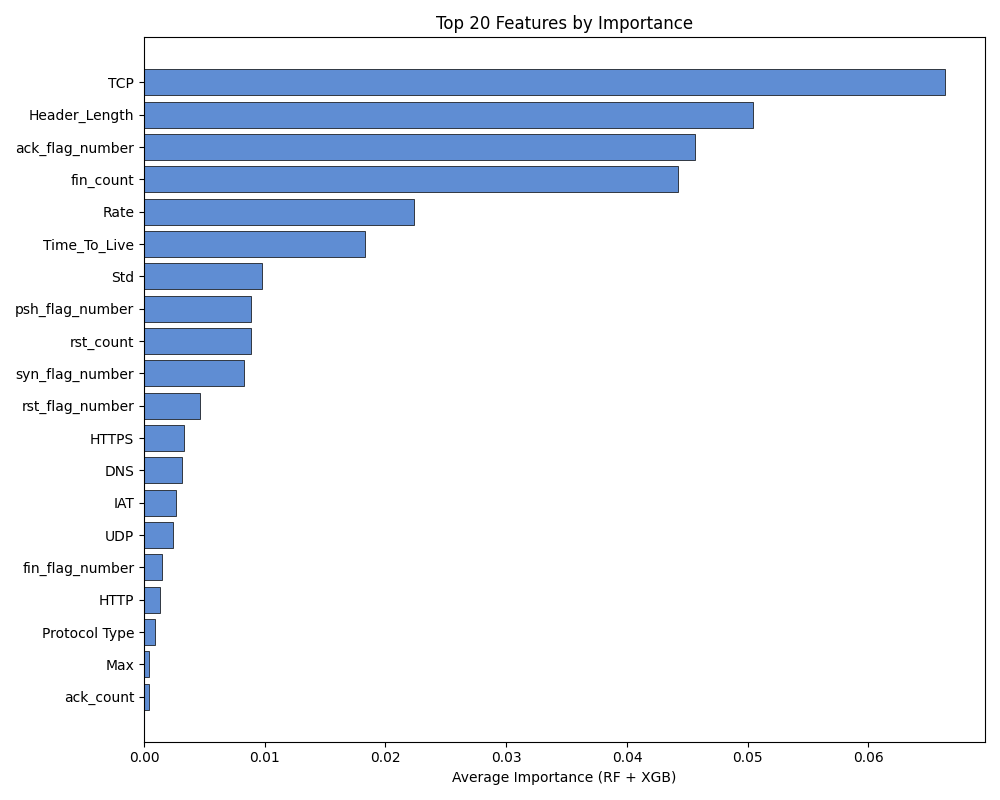
\includegraphics[width=0.55\textwidth]{figures/feature_importance.png}
    \caption{Top 20 features by permutation importance (drop in macro-F1 under feature shuffling) for the Random Forest baseline (8-class, random split).}
    \label{fig:feature_importance}
\end{figure}

\par The single most important feature by a wide margin is \texttt{Number}, the packet count within the flow window: scripted attack traffic produces highly regular packet counts that differ sharply from the variable counts of benign flows, making it the strongest single discriminator across attack families. The \texttt{HTTPS} and \texttt{HTTP} protocol indicators rank next, separating web-oriented traffic from raw-socket floods, while \texttt{Header\_Length} distinguishes protocol families at the coarsest level. The packet-length statistics (\texttt{Min}, \texttt{Max}, \texttt{Std}) and \texttt{Time\_To\_Live} contribute in the mid-range, capturing the size and network-hop signatures that help separate volumetric floods, and the TCP flag features (\texttt{psh\_flag\_number}, \texttt{syn\_flag\_number}) add handshake-pattern information. Because permutation importance here measures the drop in \emph{macro}-F1, it rewards features that help the minority application-layer classes disproportionately, which is why the broadly-informative count and protocol-indicator features outrank individual flag counts. The long low-importance tail in Figure~\ref{fig:feature_importance} confirms that the pruned 25-feature set carries little redundant signal.

\section{Model Training Dynamics}
\label{sec:training_dynamics}

\par Figure~\ref{fig:training_curves} shows the training and validation loss curves for the MLP on the random split at both the binary and 8-class granularities.

\begin{figure}[htbp]
    \centering
    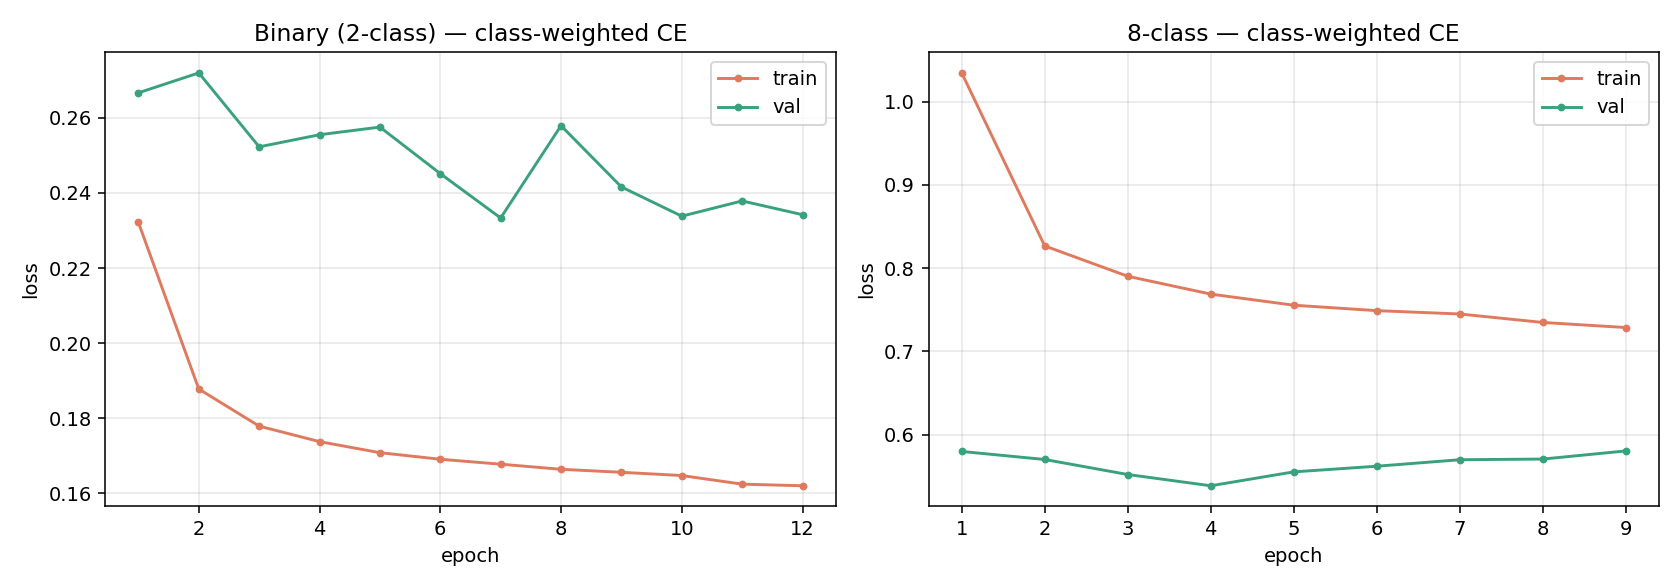
\includegraphics[width=0.66\textwidth]{figures/training_curves.png}
    \caption{MLP training and validation loss (class-weighted cross-entropy) on the random split. Left: binary (2-class) granularity. Right: 8-class granularity.}
    \label{fig:training_curves}
\end{figure}

\par The binary model reaches its best validation loss around epoch 7 and early-stops at epoch 12, and the 8-class model peaks around epoch 4 and stops at epoch 9; in both cases early stopping triggers at patience 5 after the best validation checkpoint. The loss curves show two further effects worth noting. In the binary case, the validation loss oscillates in the early epochs before settling into a stable descent, reflecting the tension between the heavily weighted minority-class gradient signals and the majority-class (DDoS) signal. In the 8-class case the validation loss sits below the training loss throughout, which is expected rather than anomalous. The training loss is computed with dropout active and batch normalisation in training mode, and is averaged over the epoch while the weights are still improving (so the epoch-1 average is inflated by the near-random early batches), whereas the validation loss is computed at the end of the epoch with dropout disabled and batch normalisation in evaluation mode. Both losses use the same class-weighted criterion, so the gap reflects this train/eval difference, not the weighting. After its epoch-4 minimum the validation loss rises while the training loss keeps falling, the onset of mild overfitting; early stopping responds by restoring the epoch-4 checkpoint, which is the model used for all reported 8-class results. The learning-rate schedule (halving on two consecutive non-improving epochs) is visible as the steeper descent segments followed by plateau phases.

\section{Binary Classification Performance}
\label{sec:binary_results}

\par Figure~\ref{fig:confusion_2class} shows the row-normalised confusion matrix for the MLP on the random-split binary (2-class) test set.

\begin{figure}[htbp]
    \centering
    \begin{minipage}[t]{0.40\textwidth}
        \centering
        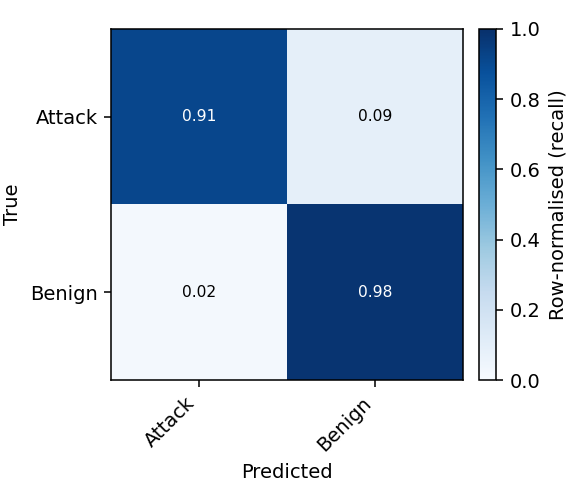
\includegraphics[width=\textwidth]{figures/confusion_2class.png}
        \caption{Row-normalised confusion matrix (per-class recall) for the MLP on the random-split 2-class test set.}
        \label{fig:confusion_2class}
    \end{minipage}\hfill
    \begin{minipage}[t]{0.56\textwidth}
        \centering
        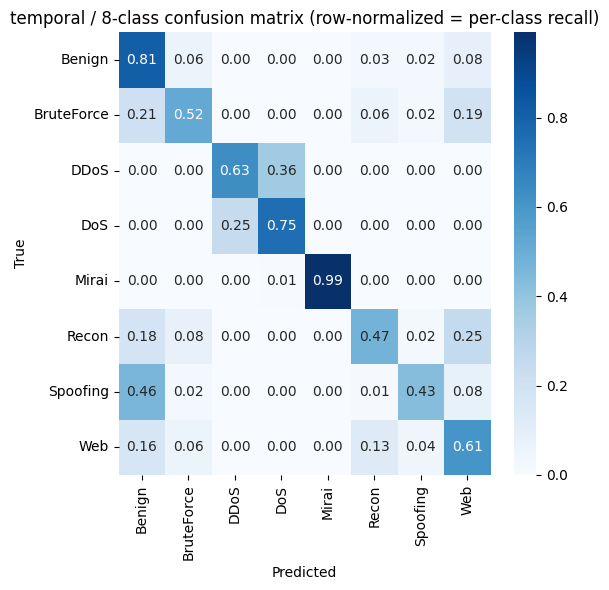
\includegraphics[width=\textwidth]{figures/confusion_8class.png}
        \caption{Row-normalised confusion matrix for the MLP on the random-split 8-class test set.}
        \label{fig:confusion_8class}
    \end{minipage}
\end{figure}

\par The binary classifier achieves high Benign recall (0.98): under 2\% of legitimate flows are falsely flagged as attacks. Attack recall is 0.91, meaning 9\% of malicious flows are missed. In a deployed IDS this trade-off is configurable via the classification threshold; the model's softmax output provides a continuous score for threshold tuning.

\section{Attack-Family Classification Performance}
\label{sec:multiclass_results}

\par Figure~\ref{fig:confusion_8class} shows the row-normalised confusion matrix for the MLP on the random-split 8-class test set.

\par Table~\ref{tab:recall_8class} summarises the per-class recall from Figure~\ref{fig:confusion_8class} alongside the main confusion targets.

\begin{table}[htbp]
\begin{center}
\begin{tabular}{|p{70pt}|p{50pt}|p{230pt}|}
\hline
\textbf{Class} & \textbf{Recall} & \textbf{Main misclassification} \\
\hline
\hline Mirai & 1.00 & None (near-perfect) \\
\hline DoS & 0.95 & 5\% predicted as DDoS \\
\hline Spoofing & 0.80 & 8\% Benign, 7\% Web \\
\hline Benign & 0.72 & 9\% BruteForce, 8\% Recon \\
\hline DDoS & 0.70 & 30\% predicted as DoS \\
\hline BruteForce & 0.62 & 18\% Web, 14\% Benign \\
\hline Recon & 0.59 & 14\% Web, 12\% BruteForce \\
\hline Web & 0.59 & 15\% BruteForce, 14\% Recon \\
\hline
\end{tabular}
\end{center}
\caption{Per-class recall on the random-split 8-class test set (MLP). Classes ordered by recall from highest to lowest.}
\label{tab:recall_8class}
\end{table}

\par The per-class recall splits into a strong and a weak group. Mirai stands apart, reaching near-perfect recall, the highest of any class, because the CICIoT2023 variants (Mirai-greith, Mirai-greip, Mirai-udpplain) all generate high-rate, fixed-payload floods over specific protocols and so produce an unusually homogeneous fingerprint that the model separates easily. The DDoS and DoS families, by contrast, are confused in both directions: both are volumetric floods differing mainly in the number of coordinated source hosts, and at the packet-feature level they share high rates, short inter-arrival times, and dominant SYN or UDP patterns, so the 30\% DDoS-to-DoS confusion (the reverse is far smaller, 5\%) is unsurprising and matches published results on similar datasets \cite{Lansky2021}. An operational IDS can tolerate this confusion, since both families call for the same response (rate-limiting and upstream filtering) and neither bleeds significantly into Benign.

\par The weaker classes are the application-layer attacks, which cluster together rather than collapsing into Benign. Brute Force (0.62 recall), Reconnaissance (0.59), and Web (0.59) are confused mainly with one another: Web with Brute Force (15\%) and Reconnaissance (14\%), Reconnaissance with Web (14\%) and Brute Force (12\%). This happens because all three are distinguished by application-layer payload content that the header-and-metadata features do not carry, leaving the model only coarse rate and size cues to tell them apart. Spoofing, by contrast, is recovered well on this run (0.80 recall), with only minor leakage to Benign (8\%) and Web (7\%). In short, the features describe how packets move, not what they carry, so the families that differ mainly in payload are the ones that remain hardest to separate from each other.

\section{Model Comparison}
\label{sec:model_comparison}

\par The same random split and evaluation protocol were applied to a Random Forest baseline. Figure~\ref{fig:weighted_f1_splits} compares weighted F1 for both models on the binary and 8-class tasks; accuracy and macro F1 are reported in Table~\ref{tab:model_comparison_table}.

\begin{figure}[htbp]
    \centering
    \begin{minipage}[t]{0.50\textwidth}
        \centering
        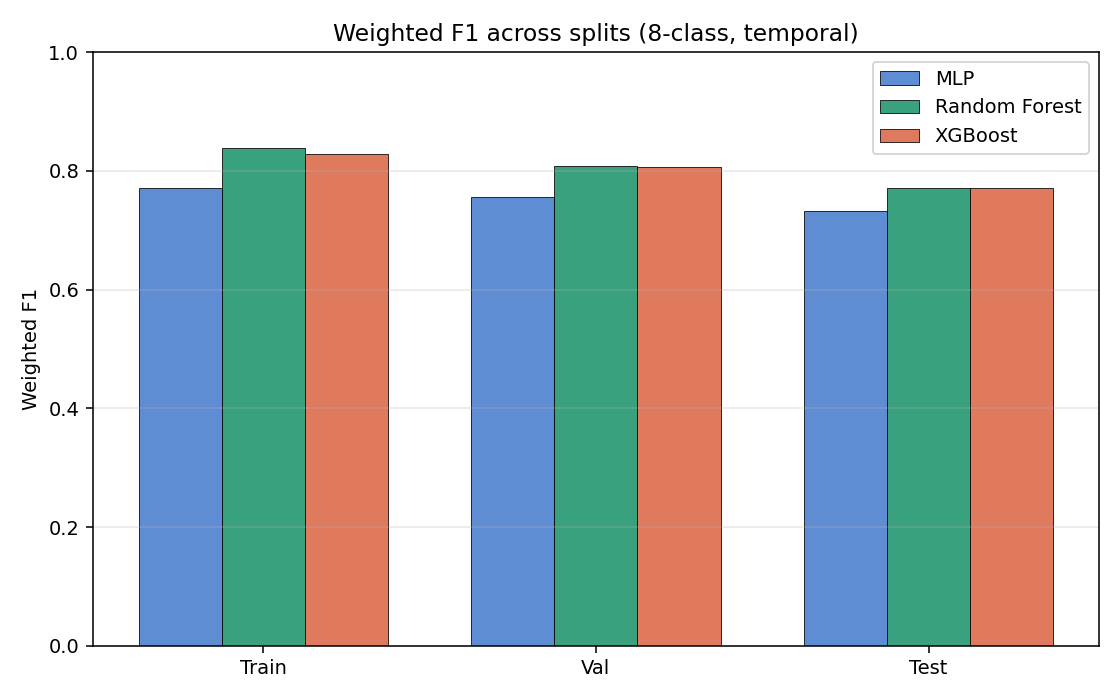
\includegraphics[width=\textwidth]{figures/weighted_f1_splits.png}
        \caption{Weighted F1 for both models on the binary and 8-class tasks (random split, test set); full metrics in Table~\ref{tab:model_comparison_table}.}
        \label{fig:weighted_f1_splits}
    \end{minipage}\hfill
    \begin{minipage}[t]{0.46\textwidth}
        \centering
        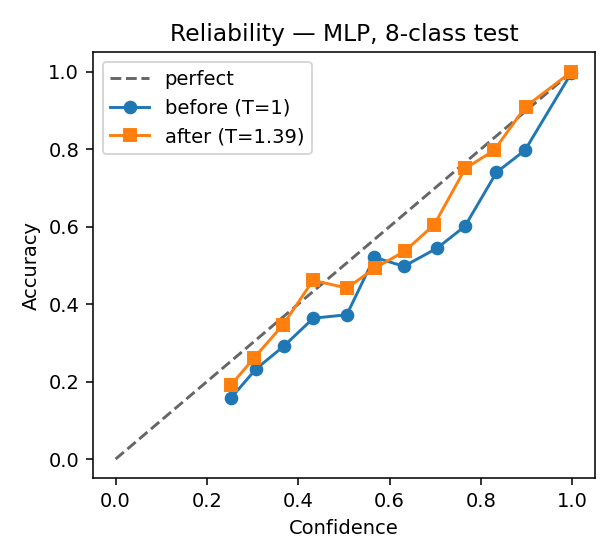
\includegraphics[width=\textwidth]{figures/reliability_8class.png}
        \caption{Reliability diagram for the MLP on the random-split 8-class test set, before and after temperature scaling.}
        \label{fig:reliability_8class}
    \end{minipage}
\end{figure}

\par Table~\ref{tab:model_comparison_table} presents the test- and validation-set metrics for the two models.

\begin{table}[htbp]
\begin{center}
\begin{tabular}{|p{65pt}|p{50pt}|p{50pt}|p{50pt}|p{55pt}|p{55pt}|}
\hline
\textbf{Model} & \textbf{Test Acc.} & \textbf{Test W-F1} & \textbf{Test Macro-F1} & \textbf{Val W-F1} & \textbf{Val Macro-F1} \\
\hline
\hline MLP & 0.775 & 0.798 & 0.631 & 0.799 & 0.632 \\
\hline Random Forest & 0.831 & 0.840 & 0.701 & 0.840 & 0.701 \\
\hline
\end{tabular}
\end{center}
\caption{Summary of key metrics on the random split (8-class granularity), held-out test set. W-F1 = weighted F1 (per-class F1 averaged by class support); Macro-F1 = unweighted (macro-averaged) F1, weighting every class equally.}
\label{tab:model_comparison_table}
\end{table}

\par Three results stand out from Table~\ref{tab:model_comparison_table}. First, no model reaches a weighted F1 of 0.85 at the 8-class granularity: the Random Forest tops out at $\approx$0.840 and the MLP at $\approx$0.798. The 0.85 acceptance bar (NFR-2, Section~\ref{sec:non_functional_requirements}) is instead met comfortably on the binary task (Section~\ref{sec:binary_results}), where weighted F1 reaches $\approx$0.93 for the MLP and $\approx$0.96 for the Random Forest; the 8-class attack-family task is reported as the harder secondary objective. Its shortfall reflects what transport-layer features can and cannot express: they do not carry the application-layer signal these families differ by (Section~\ref{sec:discussion}). The model is not the limiting factor. Second, the Random Forest outperforms the MLP by about 4 percentage points on weighted F1, 6 on accuracy, and 7 on macro F1. This result is consistent with the growing body of evidence that gradient-boosted trees and random forests are competitive (and often superior) to MLPs on tabular tasks when the sample count is in the low millions \cite{Kadra2021}. The MLP remains the primary model for the demonstration system because its inference is implemented in a single portable PyTorch call, without the additional sklearn dependency; the tree baseline serves its designed role of confirming that the deep model is not strictly worse. Third, the macro F1 gap (MLP: 0.631 vs Random Forest: 0.701) is comparable to the weighted F1 gap, and the low macro F1 of both models confirms that the difficulty is concentrated in the minority classes (particularly Web, Reconnaissance, and Brute Force), while performance on the dominant DDoS and Mirai families (which drive weighted F1) is far stronger.


\section{Confidence Calibration}
\label{sec:calibration}

\par The MLP confidences are calibrated by temperature scaling, fitting a single scalar $T$ on the validation logits and rescaling the softmax by $1/T$; the method and the Expected Calibration Error (ECE) used to measure it are defined in Section~\ref{subsec:calibration_method}. This section reports the fitted temperatures and the resulting calibration on the test set.

\par On the 8-class task the fitted temperature is $T = 1.39$, reducing ECE from 0.056 to 0.031. On the binary task the temperature is larger, $T = 2.71$, reflecting the pronounced overconfidence that class-weighted training induces on the dominant attack class, and it lowers ECE from 0.053 to 0.031. Applying the fitted temperature in the serving path therefore yields confidence scores that more faithfully reflect empirical accuracy, at zero cost to the predicted labels. Residual miscalibration remains and per-class (vector) scaling is left as future work.

\section{Discussion}
\label{sec:discussion}

\par Both models generalise from train to test with small accuracy drops (below 8 percentage points). Because the split is random, these small gaps partly reflect the within-session redundancy noted in Section~\ref{subsec:split_strategies}: many test rows have near-duplicate neighbours in training, so the figures reported here should be read as an upper bound rather than a deployment estimate.

\par The principal failure modes are the ones the design anticipated, and Section~\ref{sec:multiclass_results} traced each to the feature set rather than the model: the application-layer attacks (Web, Recon, Brute Force) leave no signal in a transport-layer representation, and the statistically similar DDoS and DoS floods overlap in feature space. Both are properties of the dataset's extraction methodology, not model defects.

\par NFR-2 (at least 0.85 weighted F1 on the \emph{binary} test set) is satisfied by both models, which reach $\approx$0.93 (MLP) to $\approx$0.96 (Random Forest). At the 8-class granularity no model reaches 0.85 (the best attain $\approx$0.84), which the design treats as the ceiling imposed by a transport-layer feature set rather than a target failure, in keeping with the secondary status assigned to the 8-class task in NFR-2. NFR-5 (faithful reporting) is respected by reporting per-class metrics rather than only aggregate numbers, so that the minority-class weakness is visible without requiring the reader to look past a high aggregate figure, and by flagging the random split's within-session redundancy (Section~\ref{subsec:split_strategies}).
